\documentclass[10pt, a4paper, landscape]{article}
\usepackage{amsmath}
\usepackage[left=2cm, right=2cm, top=2cm, bottom=2cm]{geometry}
\usepackage[colorlinks=true, urlcolor=blue]{hyperref}
\usepackage[table]{xcolor}
\usepackage{pst-all}
\usepackage{datetime}
\usepackage{threeparttable}
\usepackage{multirow}
\usepackage{pbox}
\usepackage{graphicx}

\definecolor{textRed}{HTML}{B20000}
\definecolor{backRed}{HTML}{FF8989}
\definecolor{textYellow}{HTML}{6F6E00}
\definecolor{backYellow}{HTML}{FFFF00}
\definecolor{textGreen}{HTML}{286500}
\definecolor{backGreen}{HTML}{53D000}
\definecolor{rowOne}{HTML}{F9F9F9}
%\definecolor{rowTwo}{HTML}{FFFFFF}

\newcommand{\redbox}[1]{\psframebox[linecolor=textRed, fillstyle=solid, fillcolor=backRed, framearc=0.25]{\color{textRed}{#1}}}
\newcommand{\yellowbox}[1]{\psframebox[linecolor=textYellow, fillstyle=solid, fillcolor=backYellow, framearc=0.25]{\color{textYellow}{#1}}}
\newcommand{\greenbox}[1]{\psframebox[linecolor=textGreen, fillstyle=solid, fillcolor=backGreen, framearc=0.25]{\color{textGreen}{#1}}}
\newcommand{\card}[1]{\ensuremath{\lvert #1 \rvert}}

\newdateformat{dmy}{\THEDAY\ \monthname[\THEMONTH]\ \THEYEAR}

\begin{document}
\begin{center} \huge Big-O Cheat Sheet \end{center}
%
\section*{Preface}
This is a \LaTeX'ed version of \url{http://bigocheatsheet.com/} (as of \dmy\today).
\begin{table}[h!]
\begin{tabular}{cccc} Legend: & \greenbox{Good} & \yellowbox{Fair} & \redbox{Poor} \end{tabular}
\end{table}
%
\section*{Searching}
\begin{table}[h!]
\rowcolors{1}{rowOne}{}
\begin{tabular}{lllll}
\hiderowcolors
%\hline
\multirow{2}{*}{\bf Algorithm} & \multirow{2}{*}{\bf Data Structure} & \multicolumn{2}{l}{\bf Time Complexity} & {\bf Space Complexity}\\
%\cline{3-5}
 & & {\bf Average} & {\bf Worst} & {\bf Worst}\\
%\hline
\showrowcolors
\href{http://en.wikipedia.org/wiki/Depth-first_search}{Depth First Search (DFS)} & Graph of \card{V} vertices and \card{E} edges & - & \greenbox{$O(\card{E} + \card{V})$} & \greenbox{$O(\card{V})$}\\
\href{http://en.wikipedia.org/wiki/Breadth-first_search}{Breadth First Search (BFS)} & Graph of \card{V} vertices and \card{E} edges & - & \greenbox{$O(\card{E} + \card{V})$} & \greenbox{$O(\card{V})$}\\
\href{http://en.wikipedia.org/wiki/Binary_search_algorithm}{Binary search} & Sorted array of $n$ elements & \greenbox{$O(\log n)$} & \greenbox{$O(\log n)$} & \greenbox{$O(1)$}\\
\href{http://en.wikipedia.org/wiki/Brute-force_search}{Linear (Brute Force)} & Array & \redbox{$O(n)$} & \redbox{$O(n)$} & \greenbox{$O(1)$}\\
\href{http://en.wikipedia.org/wiki/Dijkstra's_algorithm}{\pbox{\textwidth}{Shortest path by Dijkstra,\\using a Min-heap\\as priority queue}} & Graph with \card{V} vertices and \card{E} edges & \yellowbox{$O((\card{V} + \card{E}) \log \card{V})$} & \yellowbox{$O((\card{V} + \card{E}) \log \card{V})$} & \yellowbox{$O(\card{V})$}\\
\href{http://en.wikipedia.org/wiki/Dijkstra's_algorithm}{\pbox{\textwidth}{Shortest path by Dijkstra,\\using an unsorted array\\as priority queue}} & Graph with \card{V} vertices and \card{E} edges & \yellowbox{$O(\card{V}^2)$} & \yellowbox{$O(\card{V}^2)$} & \yellowbox{$O(\card{V})$}\\
\href{http://en.wikipedia.org/wiki/Bellman\%E2\%80\%93Ford_algorithm}{Shortest path by Bellman-Ford} & Graph with \card{V} vertices and \card{E} edges & \yellowbox{$O(\card{V} \card{E})$} & \yellowbox{$O(\card{V} \card{E})$} & \yellowbox{$O(\card{V})$}\\
%\hline
\end{tabular}
\end{table}
%
\clearpage
%
\section*{Sorting}
\begin{table}[h!]
\begin{threeparttable}
\rowcolors{1}{rowOne}{}
\begin{tabular}{llllll}
\hiderowcolors
%\hline
\multirow{2}{*}{\bf Algorithm} & \multirow{2}{*}{\bf Data Structure} & \multicolumn{3}{l}{\bf Time Complexity} & {\bf Worst Case Auxiliary Space Complexity}\\
%\cline{3-5}
 & & {\bf Best} & {\bf Average} & {\bf Worst} & {\bf Worst}\\
%\hline
\showrowcolors
\href{http://en.wikipedia.org/wiki/Quicksort}{Quicksort} & Array & \yellowbox{$O(n \log n)$} & \greenbox{$O(n \log n)$} & \redbox{$O(n^2)$} & \yellowbox{$O(n)$}\\
\href{http://en.wikipedia.org/wiki/Merge_sort}{Mergesort} & Array & \yellowbox{$O(n \log n)$} & \greenbox{$O(n \log n)$} & \greenbox{$O(n \log n)$} & \redbox{$O(n)$}\\
\href{http://en.wikipedia.org/wiki/Heapsort}{Heapsort} & Array & \yellowbox{$O(n \log n)$} & \greenbox{$O(n \log n)$} & \greenbox{$O(n \log n)$} & \greenbox{$O(1)$}\\
\href{http://en.wikipedia.org/wiki/Bubble_sort}{Bubble Sort} & Array & \greenbox{$O(n)$} & \redbox{$O(n^2)$} & \redbox{$O(n^2)$} & \greenbox{$O(1)$}\\
\href{http://en.wikipedia.org/wiki/Insertion_sort}{Insertion Sort} & Array & \greenbox{$O(n)$} & \redbox{$O(n^2)$} & \redbox{$O(n^2)$} & \greenbox{$O(1)$}\\
\href{http://en.wikipedia.org/wiki/Selection_sort}{Selection Sort} & Array & \redbox{$O(n^2)$} & \redbox{$O(n^2)$} & \redbox{$O(n^2)$} & \greenbox{$O(1)$}\\
\href{http://en.wikipedia.org/wiki/Bucket_sort}{Bucket sort}\tnote{a} & Array & \greenbox{$O(n+k)$} & \greenbox{$O(n+k)$} & \redbox{$O(n^2)$} & \yellowbox{$O(nk)$}\\
\href{http://en.wikipedia.org/wiki/Radix_sort}{Radix sort}\tnote{b} & Array & \greenbox{$O(nk)$} & \greenbox{$O(nk)$} & \greenbox{$O(nk)$} & \yellowbox{$O(n+k)$}\\
%\hline
\end{tabular}
\begin{tablenotes}
\item[a] Only for integers with range $k$
\item[b] Constant number of digits `$k$'
\end{tablenotes}
\end{threeparttable}
\end{table}
%
%\clearpage
%
\section*{Graphs}
\begin{table}[h!]
\rowcolors{1}{rowOne}{}
\begin{tabular}{lllllll}
\hiderowcolors
{\bf Node/Edge Management} & {\bf Storage} & {\bf Add Vertex} & {\bf Add Edge} & {\bf Remove Vertex} & {\bf Remove Edge} & {\bf Query}\\
%\hline
\showrowcolors
\href{http://en.wikipedia.org/wiki/Adjacency_list}{Adjacency list} &\yellowbox{$O(\card{V} + \card{E})$} & \greenbox{$O(1)$} & \greenbox{$O(1)$} &\yellowbox{$O(\card{V} + \card{E})$} &\yellowbox{$O(\card{E})$} &\yellowbox{$O(\card{V})$}\\
\href{http://en.wikipedia.org/wiki/Incidence_list}{Incidence list} & \yellowbox{$O(\card{V} + \card{E})$} & \greenbox{$O(1)$} & \greenbox{$O(1)$} &\yellowbox{$O(\card{E})$} &\yellowbox{$O(\card{E})$} &\yellowbox{$O(\card{E})$}\\
\href{http://en.wikipedia.org/wiki/Adjacency_matrix}{Adjacency matrix} & \redbox{$O(\card{V}^2)$} & \redbox{$O(\card{V}^2)$} & \greenbox{$O(1)$} & \redbox{$O(\card{V}^2)$} & \greenbox{$O(1)$} & \greenbox{$O(1)$}\\
\href{http://en.wikipedia.org/wiki/Incidence_matrix}{Incidence matrix} & \redbox{$O(\card{V} \card{E})$} & \redbox{$O(\card{V} \card{E})$} & \redbox{$O(\card{V} \card{E})$} & \redbox{$O(\card{V} \card{E})$} & \redbox{$O(\card{V} \card{E})$} & \yellowbox{$O(\card{E})$}\\
\end{tabular}
\end{table}
%
\clearpage
%
\section*{Data Structures}
\begin{table}[h!]
\rowcolors{1}{rowOne}{}
\begin{tabular}{llllllllll}
\hiderowcolors
\multirow{3}{*}{\bf Data Structure} & \multicolumn{8}{l}{\bf Time Complexity} & {\bf Space Complexity}\\
 & \multicolumn{4}{l}{\bf Average} & \multicolumn{4}{l}{\bf Worst} & \multirow{2}{*}{\bf Worst}\\
 & {\bf Indexing} & {\bf Search} & {\bf Insertion} & {\bf Deletion} & {\bf Indexing} & {\bf Search} & {\bf Insertion} & {\bf Deletion} & \\
\showrowcolors
\href{http://en.wikipedia.org/wiki/Array_data_structure}{Basic Array} & \greenbox{$O(1)$} & \redbox{$O(n)$} & - & - & \greenbox{$O(1)$} & \greenbox{$O(n)$} & - & - & \yellowbox{$O(n)$}\\
\href{http://en.wikipedia.org/wiki/Dynamic_array}{Dynamic Array} & \greenbox{$O(1)$} & \redbox{$O(n)$} & \redbox{$O(n)$} & \redbox{$O(n)$} & \greenbox{$O(1)$} & \redbox{$O(n)$} & \redbox{$O(n)$} & \redbox{$O(n)$} & \yellowbox{$O(n)$}\\
\href{http://en.wikipedia.org/wiki/Singly_linked_list#Singly_linked_lists}{Singly-Linked List} & \redbox{$O(n)$} & \redbox{$O(n)$} & \greenbox{$O(1)$} & \greenbox{$O(1)$} & \redbox{$O(n)$} & \redbox{$O(n)$} & \greenbox{$O(1)$} & \greenbox{$O(1)$} & \yellowbox{$O(n)$}\\
\href{http://en.wikipedia.org/wiki/Doubly_linked_list}{Doubly-Linked List} & \redbox{$O(n)$} & \redbox{$O(n)$} & \greenbox{$O(1)$} & \greenbox{$O(1)$} & \redbox{$O(n)$} & \redbox{$O(n)$} & \greenbox{$O(1)$} & \greenbox{$O(1)$} & \yellowbox{$O(n)$}\\
\href{http://en.wikipedia.org/wiki/Skip_list}{Skip List} & \yellowbox{$O(\log n)$} & \greenbox{$O(\log n)$} & \greenbox{$O(\log n)$} & \greenbox{$O(\log n)$} & \redbox{$O(n)$} & \redbox{$O(n)$} & \redbox{$O(n)$} & \redbox{$O(n)$} & \redbox{$O(n \log n)$}\\
\href{http://en.wikipedia.org/wiki/Hash_table}{Hash Table} & - & \greenbox{$O(1)$} & \greenbox{$O(1)$} & \greenbox{$O(1)$} & - & \redbox{$O(n)$} & \redbox{$O(n)$} & \redbox{$O(n)$} & \yellowbox{$O(n)$}\\
\href{http://en.wikipedia.org/wiki/Binary_search_tree}{Binary Search Tree} & \yellowbox{$O(\log n)$} & \greenbox{$O(\log n)$} & \greenbox{$O(\log n)$} & \greenbox{$O(\log n)$} & \redbox{$O(n)$} & \redbox{$O(n)$} & \redbox{$O(n)$} & \redbox{$O(n)$} & \yellowbox{$O(n)$}\\
\href{https://en.wikipedia.org/wiki/Cartesian_tree}{Cartesian Tree} & - & \greenbox{$O(\log n)$} & \greenbox{$O(\log n)$} & \greenbox{$O(\log n)$} & - & \redbox{$O(n)$} & \redbox{$O(n)$} & \redbox{$O(n)$} & \yellowbox{$O(n)$}\\
\href{http://en.wikipedia.org/wiki/B_tree}{B-Tree} & \yellowbox{$O(\log n)$} & \greenbox{$O(\log n)$} & \greenbox{$O(\log n)$} & \greenbox{$O(\log n)$} & \yellowbox{$O(\log n)$} & \greenbox{$O(\log n)$} & \greenbox{$O(\log n)$} & \greenbox{$O(\log n)$} & \yellowbox{$O(n)$}\\
\href{http://en.wikipedia.org/wiki/Red-black_tree}{Red-Black Tree} & \yellowbox{$O(\log n)$} & \greenbox{$O(\log n)$} & \greenbox{$O(\log n)$} & \greenbox{$O(\log n)$} & \yellowbox{$O(\log n)$} & \greenbox{$O(\log n)$} & \greenbox{$O(\log n)$} & \greenbox{$O(\log n)$} & \yellowbox{$O(n)$}\\
\href{https://en.wikipedia.org/wiki/Splay_tree}{Splay Tree} & - & \greenbox{$O(\log n)$} & \greenbox{$O(\log n)$} & \greenbox{$O(\log n)$} & - & \greenbox{$O(\log n)$} & \greenbox{$O(\log n)$} & \greenbox{$O(\log n)$} & \yellowbox{$O(n)$}\\
\href{http://en.wikipedia.org/wiki/AVL_tree}{AVL Tree} & \yellowbox{$O(\log n)$} & \greenbox{$O(\log n)$} & \greenbox{$O(\log n)$} & \greenbox{$O(\log n)$} & \yellowbox{$O(\log n)$} & \greenbox{$O(\log n)$} & \greenbox{$O(\log n)$} & \greenbox{$O(\log n)$} & \yellowbox{$O(n)$}\\
\end{tabular}
\end{table}
%
%\clearpage
%
\section*{Heaps}
\begin{table}[h!]
\begin{threeparttable}
\rowcolors{1}{rowOne}{}
\begin{tabular}{llllllll}
\hiderowcolors
\multirow{2}{*}{\bf Heaps} & \multicolumn{7}{l}{\bf Time Complexity}\\
 & {\bf Heapify} & {\bf Find Max} & {\bf Extract Max} & {\bf Increase Key} & {\bf Insert} & {\bf Delete} & {\bf Merge}\\
\showrowcolors
\href{http://en.wikipedia.org/wiki/Linked_list}{Linked List (sorted)} & - & \greenbox{$O(1)$} & \greenbox{$O(1)$} & \redbox{$O(n)$} & \redbox{$O(n)$} & \greenbox{$O(1)$} & \redbox{$O(m+n)$}\\
\href{http://en.wikipedia.org/wiki/Linked_list}{Linked List (unsorted)} & - & \redbox{$O(n)$} & \redbox{$O(n)$} & \greenbox{$O(1)$} & \greenbox{$O(1)$} & \greenbox{$O(1)$} & \greenbox{$O(1)$}\\
\href{http://en.wikipedia.org/wiki/Binary_heap}{Binary Heap} & \yellowbox{$O(n)$} & \greenbox{$O(1)$} & \yellowbox{$O(\log n)$} & \yellowbox{$O(\log n)$} & \yellowbox{$O(\log n)$} & \yellowbox{$O(\log n)$} & \redbox{$O(m + n)$}\\
\href{http://en.wikipedia.org/wiki/Binomial_heap}{Binomial Heap} & - & \yellowbox{$O(\log n)$} & \yellowbox{$O(\log n)$} & \yellowbox{$O(\log n)$} & \yellowbox{$O(\log n)$} & \yellowbox{$O(\log n)$} & \yellowbox{$O(\log n)$}\\
\href{http://en.wikipedia.org/wiki/Fibonacci_heap}{Fibonacci Heap} & - & \greenbox{$O(1)$} & \yellowbox{$O(\log n)$}\tnote{a} & \greenbox{$O(1)$}\tnote{a} & \greenbox{$O(1)$} & \yellowbox{$O(\log n)$}\tnote{a} & \greenbox{$O(1)$}\\
\end{tabular}
\begin{tablenotes}
\item[a] Amortized
\end{tablenotes}
\end{threeparttable}
\end{table}
%
%\clearpage
%
\section*{Big-O Complexity Chart}
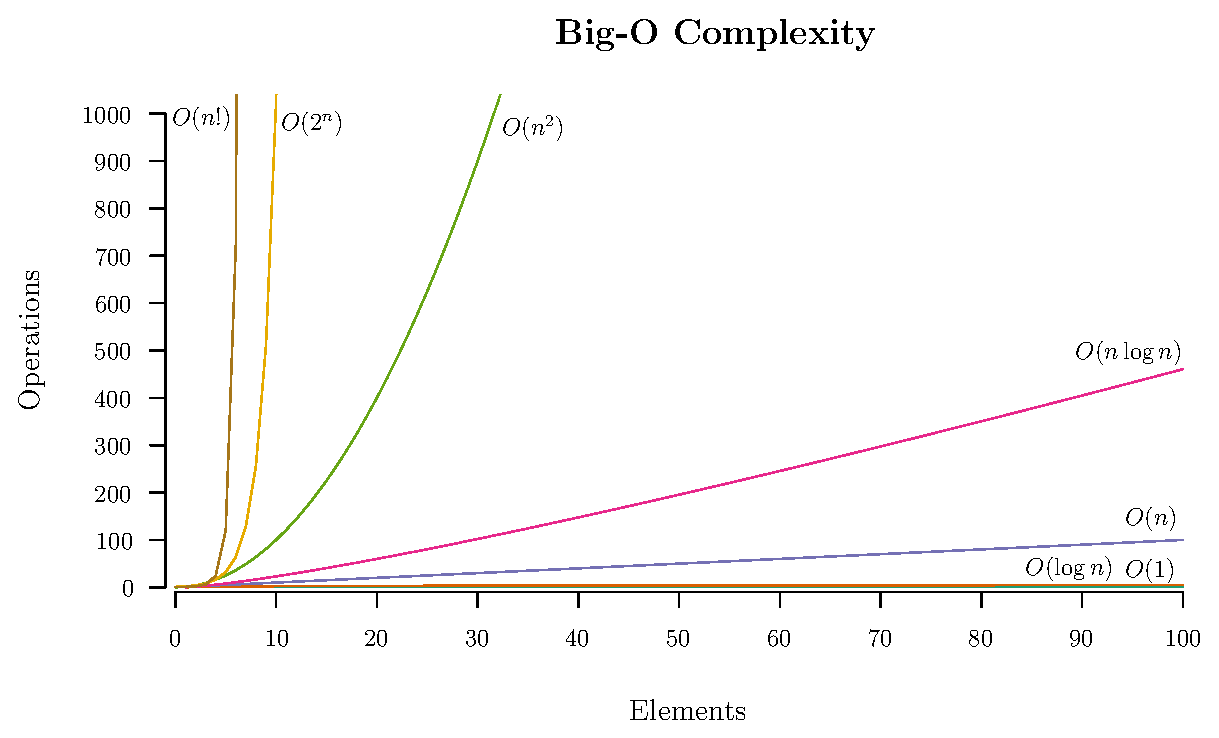
\includegraphics{Big-O.eps}
\end{document}